  \documentclass{article}
\usepackage[utf8]{inputenc}
\usepackage[top=3cm, bottom=3cm, left=3cm,right=3cm]{geometry}
%\usepackage[numbers,round]{natbib}
\usepackage{natbib}
\setcitestyle{aysep={}} 
\usepackage{graphicx}
\usepackage{color}
\usepackage{amsfonts}
\usepackage{setspace}
\usepackage{amsmath}
\usepackage{mathtools}
\usepackage{bbm}
\usepackage{float}
\usepackage{hyperref}
\usepackage[super]{nth}
\usepackage{tikzit}
\input{fig.tikzstyles}
\usepackage{algorithm}  
\usepackage{algpseudocode}

\parindent0cm
\parskip0.5cm
\hyphenpenalty=10000
\pretolerance=10000
\usepackage{lineno}
\linespread{1.5}

% Line numbering works around align environment without requiring paragraph break
\let\oldalign\align
\let\oldendalign\endalign
\renewenvironment{align}{\linenomathNonumbers\oldalign}{\oldendalign\endlinenomath}

\linenumbers

\makeatletter
\newcommand{\customlabel}[2]{
\protected@write \@auxout {}{\string \newlabel {#1}{{#2}{}}}}
\makeatother

%\renewcommand\footnote[2][]{\relax}
\renewcommand{\eqref}[1]{\ref{#1}}

\begin{document}
{\Large An unconstrained Euclidean parametrisation of phylogenetic tree space}

\vspace*{2cm}
Xavier Didelot$^{1,2,*}$

\vspace*{2cm}
$^1$ School of Life Sciences, University of Warwick, Coventry, United Kingdom\\
$^2$ Department of Statistics, University of Warwick, Coventry, United Kingdom\\
$^*$ Corresponding author. Tel: 0044 (0)2476 572827. Email: \verb+xavier.didelot@warwick.ac.uk+

\vspace*{2cm}
Running title: Euclidean parametrisation of phylogenetic trees

\vspace*{2cm}
Keywords: phylogenetic trees; Euclidean parametrisation; 
ultrametric trees; rooted trees; unrooted trees

%\newpage
%\section*{Abstract}

\newpage
\section{Introduction}

Phylogenetic trees are usually represented using two components: 
the topology of the tree which is discrete and the branch lengths of the tree
which are continuous \citep{Paradis2006}. 
This mixed nature makes it difficult to explore the 
tree space, using for example moves such as 
nearest-neighbor interchange (NNI)
or subtree pruning and regrafting (SPR). However, these moves are not easy to optimise \citep{hohnaGuidedTreeTopology2012,zhangUsingParsimonyGuidedTree2020}. 

The Billera‐Holmes‐Vogtmann (BHV) 
tree space \citep{Billera2001} is made of one orthant
for each topology, connected between themselves at the points where a branch length degenerates
to zero to switch from one topology to another. The BHV space is continuous,
but its geometry is complex and intrinsically linked with the nature of phylogenetic trees.
Consequently, using the BHV 
is difficult and requires specialised algorithms 
\citep{dinhProbabilisticPathHamiltonian2017}. 

Here we propose a new unconstrained Euclidean parametrisation of phylogenetic
trees, with fixed number of dimensions, equal to the number of parameters required to specify the 
branch lengths of a phylogenetic tree.
This parametrisation represents topology and branch lengths in a single unconstrained Euclidean space, permitting continuous paths between topologies and providing a foundation for the development of continuous-space computational methods.

The remainder of this article is structured as follows.
First we present the general recursive principle used
for all constructions, using contour traversal for grafting
leaves one by one. Next we show how this can be applied
for ultrametric rooted trees, general rooted trees and
unrooted trees, respectively. Finally we show numerical
validation of the three proposed constructions.

\section{Recursive contour-grafting construction}

All our parametrisations are constructed recursively using the
same basic principle.
We consider an arbitrary but fixed order for the leaves.
The tree is constructed by adding each
leaf one by one to the tree built so far. 
Let $T_i$ denote the rooted tree formed by the first $i$ leaves and let
$L(T_i)$ be the sum of the branch lengths in the tree $T_i$.
The tree $T_1$ consists only of the first leaf.
When adding
each leaf $i$ beyond the first one, 
a graft point $x_i$ is selected on or above $T_{i-1}$
corresponding to the point
where the new leaf is attached. 
This process is repeated for all leaves from the second one ($i=2$) to the last one ($i=n$), each time
adding to the tree $T_{i-1}$ built previously.

The location of a
graft point $x_i$ is parametrised using a variable $a_i \in \mathbb{R}$.
If $0\leq a_i \leq 2L(T_{i-1})$ then $a_i$ corresponds to the distance travelled
along the contour traversal of $T_{i-1}$ before reaching the graft point.
Starting at the root, the traversal follows each branch once away from the root and 
once back towards it, visiting the first child of each internal node and then the second. 
Let $|T|$ denote the set of points on the tree $T$.
The process of finding this graft point on a tree $T$ using the contour traversal is denoted:
\begin{equation}
\label{eq:contour}
\gamma_T: [0,2L(T)] \rightarrow |T|%, a \rightarrow \gamma_T(a)
\end{equation}

We further define the extended contour traversal as illustrated in 
in Figure \ref{fig:contour} and described below.
If $a_i>2L(T_{i-1})$, the grafting point is above the root of $T_{i-1}$ by length $a_i-2L(T_{i-1})$.
Likewise, if $a_i<0$ then the grafting point is above the root of $T_{i-1}$ by length $-a_i$.
This extended contour traversal is therefore a function $\Gamma_{T}: \mathbb{R} \rightarrow
|T|^+$. The co-domain $|T|^+$ is obtained by adding to $|T|$ the points on a branch above
the root at a distance $d \in [0,\infty)$, with zero identified with the root. 
The extended contour traversal is defined as:
\begin{equation}
\label{eq:contour-extended}
\Gamma_{T}(a)=
\begin{cases} 
      \text{point above root by }-a & \text{if } a<0 \\ 
      \gamma_{T}(a) & \text{if } 0\leq a \leq 2L(T) \\ 
      \text{point above root by }a-2L(T) &\text{if }a>2L(T) 
   \end{cases}
\end{equation}

\begin{figure}[t]
\ctikzfig{fig1}
\caption{Illustration of the contour traversal. The initial tree is shown in black, with three 
leaves labeled 1, 2 and 3 and all four branches of length 1.
Leaf 4 is added with the value of $a_4$ determining the graft point as shown and the new terminal branch
shown in red.
\label{fig:contour}}
\end{figure}

At the graft point $x_i=\Gamma_{T_{i-1}}(a_i)$, 
a new node is created with first child equal to what was previously below that point,
and second child equal to the new branch of length $\ell_i$ leading to the leaf $i$.
This convention also defines the ordering of the children used in subsequent contour traversals.

The extended contour traversal is continuous because $\gamma_T(0)=\gamma_T(2(L(T))=\mathrm{root}(T)$. Every point in the interior of an edge of $T$ is visited exactly twice, once in each
traversal direction. A point at distance $d>0$ above the root also has exactly two preimages,
namely $-d$ and $2L(T)+d$.
We can deduce the following recursive formula for the sum of the branch lengths $L(T_i)$:
\begin{equation}
L(T_i)=\begin{cases}
0 & \text{if $i=1$}\\
L(T_{i-1})+\ell_i+\mathrm{max}(0,a_i-2L(T_{i-1}))+\mathrm{max}(0,-a_i) & \text{otherwise}
\end{cases}
\end{equation}


\section{Rooted ultrametric trees}

We consider phylogenetic trees that are binary, ultrametric and rooted, 
with $n$ labeled leaves. 
There are $n-1$ internal nodes including the root.
The topology of the tree is 
discrete and there are 
$(2n-3)!!=(2n-2)!/(2^{n-1}(n-1)!)$ unique possibilities \citep{Felsenstein1978b}. 
The branch lengths are continuous but not independent from each other.
Since the tree is ultrametric, the branch lengths are constrained
so that the number of free parameters corresponds to the $n-1$ values
for the heights of the internal nodes relative to the contemporaneous leaves.

The previous section introduced the recursive principle for constructing
trees using the extended contour traversal for grafting, with 
parameters $(a_i)_{i=2,...,n} \in \mathbb{R}^{n-1}$ used in Equation \ref{eq:contour-extended}.
This construction is necessary and sufficient to define an ultrametric
rooted tree, since once a graft point has been selected, the newly created
terminal branch must stretch from the graft point to the contemporaneous
time in which all leaves belong. In particular, the dimensionality of the parameters
is $n-1$ which is the dimensionality needed to specify the 
$n-1$ heights of the internal nodes. 
For a point $x$ on an ultrametric tree, let $h_T(x)$ denote its distance to any descendant leaf.
For a point at distance $d$ above the current root $r$, its distance is $h_T(x)=h_T(r)+d$. 

Let $\mathcal{C}_n^1=\mathbb{R}^{n-1}$ denote the parameter space defined above and let
$\mathcal{T}_n^1$ denote the space of ultrametric phylogenetic trees with $n$ labelled leaves. 
An element of $\mathcal{C}_n^1$
is the vector $C=(a_i)_{i=2,...,n}$ and it defines a unique phylogenetic tree $T\in\mathcal{T}_n$.
This construction defines a function $\Phi_n^1:\mathcal{C}_n^1\rightarrow\mathcal{T}_n^1$,
which is detailed in Algorithm \ref{alg:decoding1}. This function is surjective, 
meaning that for any phylogenetic tree $T$ there is at least
one parametrisation $C$ such that $\Phi_n^1(C)=T$. 
To see this, consider any $T\in\mathcal{T}_n^1$, remove leaf $n$ and its pendant branch, 
and suppress its resulting degree-two parent. 
Repeating this operation produces trees with successively fewer leaves. Reversing these steps reconstructs $T$ using the proposed grafting procedure, because every required grafting location is reached by the contour traversal and every terminal branch length $\ell_i>0$ is deterministic.
However, the function $\Phi_n^1$ is not injective as there
are more than one $C$ such that $\Phi_n^1(C)=T$. This is a consequence of each grafting point being
visited twice by the contour traversal: once as the algorithm goes down the branch and then
again as it goes back up the branch. Likewise, a grafting point above the root by length $x$
can be obtained by both $a_i=-x$ and $a_i=2L(T_{i-1})+x$.
Each grafting point is therefore represented exactly twice if we exclude the possibility of branches
of length zero. 
For an ultrametric rooted binary tree $T$ with strictly positive branch lengths, there are therefore $2^{n-1}$ 
distinct values of $C$ such that $\Phi_n^1(C)=T$.
The duplication of grafting coordinates is needed to achieve continuity: it allows the grafting location 
to move continuously through the endpoints of the contour and across changes in tree topology, without 
an explicit jump between discrete topological states.

\begin{algorithm}
\caption{Parametrisation of ultrametric rooted trees}
\label{alg:decoding1}
\begin{algorithmic}[1]
\Require Ordered leaves $1,\ldots,n$ and parameters
         $C=(a_i)_{i=2,...,n}\in\mathbb{R}^{n-1}$
\Ensure An ultrametric rooted phylogenetic tree $T_n$
\State Let $T_1$ consist of the single leaf $1$, which is also its root
\State $L(T_1)\gets 0$
\For{$i=2,\ldots,n$}
   \State Find the grafting point $x_i=\Gamma_{T_{i-1}}(a_i)$ using Equation \ref{eq:contour-extended}
    \State If $x_i$ lies above the current root, let $x_i$ be the new root
    \State Insert a new internal node at $x_i$, splitting its branch if necessary
    \State Make the subtree previously below $x_i$ the first child of this node
    \State Attach leaf $i$ as its second child by a branch of length $\ell_i=h_{T_{i-1}}(x_i)$
    \State Denote the resulting tree by $T_i$
    \State $L(T_i)\gets L(T_{i-1})+\ell_i
          +\max(0,-a_i)+\max(0,a_i-2L(T_{i-1}))$
\EndFor
\State \Return $T_n$
\end{algorithmic}
\end{algorithm}

To show mathematically that the parametrisation is continuous, we need to consider
a tree space with a well-defined associated metric.
Let $\mathcal{B}_n^1$ denote the appropriate Billera‐Holmes‐Vogtmann (BHV) 
tree space \citep{Billera2001} of rooted ultrametric 
phylogenetic trees with $n$ labelled leaves
including trees with zero-length internal branches. The Algorithm \ref{alg:decoding1} can be seen as
defining a function $\Phi_n^1:\mathcal{C}_n^1 \rightarrow \mathcal{B}_n^1$ which is continuous.
Within each region of parameter space in which the selected contour segments and traversal directions are fixed, all node heights and branch lengths vary continuously with the parameters $a_i$. 
When a grafting location passes through an internal node, the separating internal branch contracts continuously to zero before the adjacent topology is entered. Both topologies therefore meet at the same boundary tree in BHV space. The extension above the root also tends continuously to zero when 
$a_i$ approaches either endpoint of the contour ($a_i=0$ and $a_i=2L(T_{i-1}))$.
Applying this argument recursively at each grafting step establishes the continuity of $\Phi_n^1$.

Finally we calculate the Jacobian of the function
$\Phi_n^1: \mathcal{C}_n^1 \rightarrow \mathcal{T}_n^1$.
Let $\boldsymbol{h}=(h_2,...,h_n)$ where $h_i$ is the height of the internal node
created when leaf $i$ is grafted. Within a fixed contour region, $h_i=h_{T_{i-1}}(\Gamma_{T_{i-1}}(a_i))$.
The new height depends only on $a_2,...,a_i$, not on later parameters. Moreover,
$$
\frac{\partial h_i}{\partial a_i}\in \{-1,+1\}
$$
because height changes at unit rate along every fixed contour segment and along the branch
above the root. Therefore the Jacobian matrix is triangular, with diagonal entries $+1$ or $-1$, and
$$
\left|
\det\frac{\partial(h_2,...,h_n)}
{\partial(a_2,...,a_n)}
\right|=1
$$

Given a density $p_T$ on ultrametric tree space, a natural symmetric pullback assigns equal
mass to the $2^{n-1}$ representations of each generic tree. Since the absolute Jacobian is one, 
the corresponding density on $C$ is:
\begin{equation}\label{eq:tree-distrib1}
p_C(C) = 
\frac{1}{2^{n-1}}
p_T(\Phi_n^1(C))
\end{equation}

\section{Rooted trees with unrestricted branch lengths}

We consider phylogenetic trees that are binary and rooted, with $n$ labeled leaves. 
There are $n-1$ internal nodes including the root.
The topology of the tree is 
discrete and there are 
$(2n-3)!!=(2n-2)!/(2^{n-1}(n-1)!)$ unique possibilities \citep{Felsenstein1978b}. 
The branch lengths are continuous, and there are $2n-2$ branch lengths
taking values in $\mathbb{R}_{>0}$ (one for each leaf and non-root internal node). 
Our construction is similar to the one above for ultrametric trees. 
The main difference is that there is now another parameter $b_i \in \mathbb{R}$
for each leaf beyond the first one, that represents the length 
$\mathrm{exp}(b_i)$ of the branch
separating the graft point (determined by $a_i$) and the newly added leaf $i$.

Let $\mathcal{C}_n^2=\mathbb{R}^{2n-2}$ denote the parameter space defined above and let
$\mathcal{T}_n^2$ denote the space of rooted phylogenetic trees with $n$ labelled leaves. 
An element of $\mathcal{C}_n^2$
is the vector $C=((a_i,b_i))_{i=2,...,n}$ and it defines a unique phylogenetic tree $T\in\mathcal{T}_n^2$.
The construction above defines a function $\Phi_n^2:\mathcal{C}_n^2\rightarrow\mathcal{T}_n^2$,
which is detailed in Algorithm \ref{alg:decoding2}. 
Following the same arguments as outlined above for ultrametric
trees, we can show that this function is continuous and surjective. It is not injective, instead
each rooted binary tree with strictly positive branch lengths has exactly $2^{n-1}$ preimages.

\begin{algorithm}
\caption{Parametrisation of rooted phylogenetic trees}
\label{alg:decoding2}
\begin{algorithmic}
\Require Ordered leaves $1,\ldots,n$ and parameters
         $C=((a_i,b_i))_{i=2,...,n}\in\mathbb{R}^{2n-2}$
\Ensure A rooted phylogenetic tree $T_n$
\State Let $T_1$ consist of the single leaf $1$, which is also its root
\State $L(T_1)\gets 0$
\For{$i=2,\ldots,n$}
   \State Find the grafting point $x_i=\Gamma_{T_{i-1}}(a_i)$ using Equation \ref{eq:contour-extended}
    \State If $x_i$ lies above the current root, let $x_i$ be the new root
    \State Insert a new internal node at $x_i$, splitting its branch if necessary
    \State Make the subtree previously below $x_i$ the first child of this node
    \State Attach leaf $i$ as its second child by a branch of length $\exp(b_i)$
    \State Denote the resulting tree by $T_i$
    \State $L(T_i)\gets L(T_{i-1})+\exp(b_i)
          +\max(0,-a_i)+\max(0,a_i-2L(T_{i-1}))$
\EndFor
\State \Return $T_n$
\end{algorithmic}
\end{algorithm}

As previously, we calculate the Jacobian of the function
$\Phi_n^2: \mathcal{C}_n^2 \rightarrow \mathcal{T}_n^2$.
We consider this Jacobian locally, within a region of \(\mathcal C_n\) where the resulting topology and the branch containing each grafting point are fixed. Let \(\boldsymbol\ell^{(i-1)}\) denote the vector of branch lengths in \(T_{i-1}\). If leaf \(i\) is grafted in the interior of a branch of length \(\ell_j\), that branch is replaced by two branches of lengths
\[
u_i(\boldsymbol\ell^{(i-1)},a_i)
\quad\text{and}\quad
\ell_j-u_i(\boldsymbol\ell^{(i-1)},a_i)
\]
and a terminal branch of length \(\exp(b_i)\) is added. Along any fixed segment and direction of the contour traversal, \(u_i\) is affine in \(a_i\), with
\[
\frac{\partial u_i}{\partial a_i} \in \{-1,1\}
\]
After reordering the branch-length coordinates, the absolute Jacobian determinant of this grafting step is therefore
\[
\left|
\det\frac{\partial\boldsymbol\ell^{(i)}}
{\partial(\boldsymbol\ell^{(i-1)},a_i,b_i)}
\right|
=
\left|\frac{\partial u_i}{\partial a_i}\right|
\frac{\partial\exp(b_i)}{\partial b_i}
=\exp(b_i)
\]
The same result holds when the grafting point lies above the root, since the new root branch has derivative $-1$ or $+1$ with respect to $a_i$. Applying recursively gives, for every $C$ in which the grafting points do not coincide with a node or an endpoint of the contour:
\begin{equation*}
\left|
\det\frac{\partial\boldsymbol\ell(\Phi_n(C))}{\partial C}
\right|
=\prod_{i=2}^n\exp(b_i)
=\exp\!\left(\sum_{i=2}^n b_i\right)
\end{equation*}

Given a density $p_T$ on rooted tree space, a natural symmetric pullback assigns
equal mass to the $2^{n-1}$ representations of each generic tree. The corresponding density on $C$ is therefore: 
\begin{equation}\label{eq:tree-distrib2}
p_C(C) = p_T(\Phi_n^2(C))
\frac{1}{2^{n-1}}\mathrm{exp}\left( \sum_{i=2}^n b_i\right)
\end{equation}

\section{Unrooted trees}

TODO using the unextended contour traversal in Equation \ref{eq:contour}.

\section{Numerical validation}

We consider rooted trees, such that all of the $(2n-3)!!$ topologies are equally
likely and the branch lengths $\ell_i$ follow an Exponential distribution with mean $\theta$, so that:
\begin{equation}\label{eq:tree-distrib0}
p_T(T)=\frac{1}{(2n-3)!!}\prod_{i=1}^{2n-2}\theta^{-1}\exp\left(-\frac{\ell_i}{\theta}\right)
\end{equation}

To sample from this distribution, we use the adaptive Metropolis sampler \citep{Vihola2011}. 
This algorithm uses a multivariate normal distribution as the proposal kernel
$q(C'|C)$ which is symmetric ($q(C'|C)=q(C|C')$), so that the acceptance probability 
is simply $\mathrm{min}(1,p_C(C')/p_C(C))$ calculated using Equation \ref{eq:tree-distrib2}.
The mean of the proposal kernel is the current value $C$ and 
its covariance matrix is tuned to achieve an acceptance
rate of 0.234 \citep{Andrieu2008}. 
We take $n=5$ as a small example, with $\theta=2$ as the mean of the distribution of branch lengths.
The sampler was run for $2\times10^{5}$ iterations, with the first half discarded
as burn-in and the remainder sampled every 100 iterations to produce a sample
of size 1000. This run took less than a minute on a standard laptop. 
Figure \ref{fig:mcmc} shows that the trees sampled by the MCMC are distributed as 
expected under Equation \ref{eq:tree-distrib0}. All $(2n-3)!!=105$ topologies have been sampled,
the distribution of the sum of branch lengths and of a single branch length are as expected,
and a majority-rule consensus tree looks completely star-like. The effective sample size
was greater than 200 for individual branch lengths as computed using the R
package coda \citep{Plummer2006}. The approximate effective sample size
of the tree topology was also greater than 200 as computed by the R package
rwty \citep{Warren2017}.

\begin{figure}[p!]
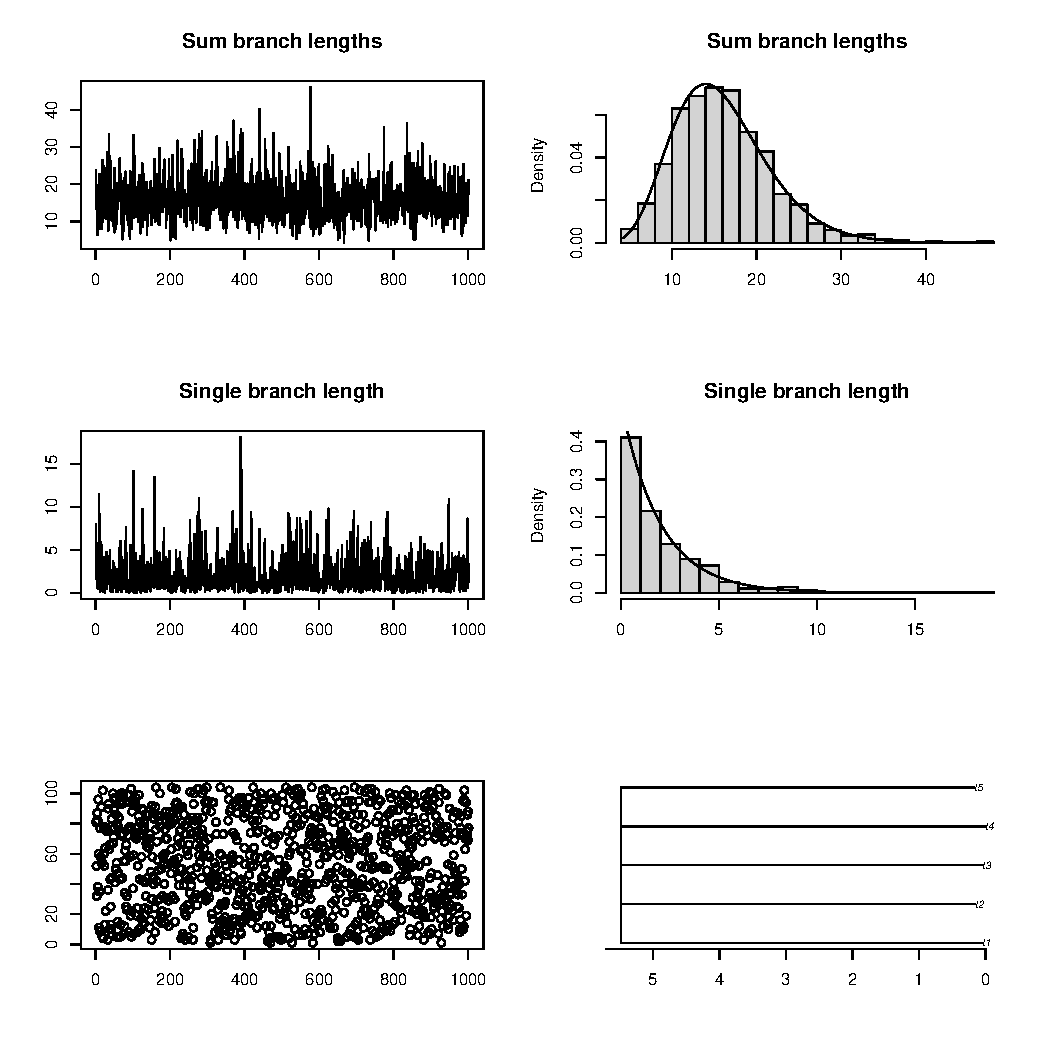
\includegraphics{mcmc}
\caption{MCMC run. 
(A) Trace of sum of branch lengths.
(B) Distribution of sum of branch lengths, sampled (histogram) and expected (line).
(C) Trace of a single branch length.
(D) Distribution of a single branch length, sampled (histogram) and expected (line).
(E) Trace of topology.
(F) Majority-rule consensus tree.
\label{fig:mcmc}}
\end{figure}

\section{Discussion}

The aim of Bayesian phylogenetic inference is to reconstruct
a tree given some genetic data using Bayesian statistics to capture
the posterior distribution of the tree \citep{nascimentoBiologistsGuideBayesian2017}.
This is usually done using a Markov Chain Monte-Carlo (MCMC) 
to generate samples from this posterior distribution \citep{Gilks1996}. 
The MCMC needs to propose updates
to both the branch lengths and the topology, with the latter using topology-changing moves such as 
nearest-neighbor interchange (NNI)
or subtree pruning and regrafting (SPR). However, these moves are not easy to optimise \citep{hohnaGuidedTreeTopology2012,zhangUsingParsimonyGuidedTree2020}. 
Conversely, many promising MCMC methods have not been applied in Bayesian phylogenetics
because they can only be applied to continuous parameters. 
This includes in particular some adaptive methods where proposal parameters are learned 
during sampling \citep{Andrieu2008}, as well as gradient-based approaches such as 
the Langevin and Hamiltonian methods \citep{robertsOptimalScalingDiscrete1998,nealMCMCUsingHamiltonian2011,Betancourt2017}. 
For example the dynamic Hamiltonian Monte Carlo (HMC) method implemented in Stan
\citep{Carpenter2017,Betancourt2017}.
After observing data $D$ made of $n$ aligned genetic sequences of length $l$, the 
distribution becomes the posterior with density
$%\begin{equation}\label{eq:posterior}
p_C(C|D) \propto p_C(C) p(D|T=\Phi_n(C))
$%\end{equation}
where the last term is the likelihood of the data given the phylogenetic tree $T=\Phi_n(C)$
obtained using Algorithm \ref{alg:decoding2}. This likelihood can be calculated efficiently
using the Felsenstein pruning algorithm \citep{Felsenstein1981} which is used in
most phylogenetic inference tools. Many substitution models can be used to calculate
this likelihood \citep{nascimentoBiologistsGuideBayesian2017} and here we use the simplest 
Jukes-Cantor model \citep{Jukes1969} which avoids having to infer additional
parameters.

\clearpage
\bibliographystyle{elsarticle-harv}
\IfFileExists{/Users/u1775021/all.bib}
{\bibliography{/Users/u1775021/all.bib}}
{\bibliography{biblio}}

\end{document}

